\begin{center}		
\begin{tikzpicture}
		
		
			\begin{axis}[/pgf/number format/.cd, use comma,1000 sep={\,},
				width=13cm,height=13cm,
				xmin=-3.4,xmax=4.4,ymin=-12.7,ymax=5.2,
				xtick={-4,-3,...,5},
				minor x tick num =4,
				ytick={-14,-13,...,5},
				minor y tick num =4,
				tick label style={font=\scriptsize},
				grid=both, axis lines=center,
				grid style={gray!35,line width=0.3pt},
				minor grid style={gray!20,line width=0.2pt},
				enlargelimits=false]
				\addplot[color=blue,domain=-3:4,smooth,samples=200,line width=1.2pt] {-1*(x+1)*(x-3)} node [above right,pos=0.8] {$\mathcal{C}_f$};
				\node[below left] at (axis cs:0,0) {\scriptsize 0};			
				\coordinate[label=135:A] (A) at (axis cs:-2,-5) ;
				\node[draw=black,thick,rotate=45,cross out,inner sep=0pt,minimum width=3pt,minimum height=3pt] at (A) {};
				\coordinate[label=135:C] (C) at (axis cs:-1,1) ;
				\node[draw=black,thick,rotate=45,cross out,inner sep=0pt,minimum width=3pt,minimum height=3pt] at (C) {};
				\coordinate[label=90:B] (B) at (axis cs:1,4) ;
				\node[draw=black,thick,rotate=45,cross out,inner sep=0pt,minimum width=3pt,minimum height=3pt] at (B) {};
				\addplot[color=red,domain=-5:6,smooth,samples=2,line width=1pt] {-5+6*(x+2)} node [above left,pos=0.38] {$(d)$};
				\addplot[color=green4,domain=-5:6,smooth,samples=2,line width=1pt] {4} node [above left,pos=0.65] {$T$};
			\end{axis}
				
		\end{tikzpicture}
\end{center}



On considère la courbe représentative $\mathcal{C}_f$ d'une fonction $f$ définie sur l'intervalle $[-3\,;\,4]$.\par
On note $f'$ la fonction dérivée de la fonction $f$.

On précise que :
\begin{itemize}
\item la droite $(d)$ est tangente à la courbe $\mathcal{C}_f$ au point A et passe par le point C ;
\item la tangente à $C_f$ au point B est parallèle à l'axe des abscisses.
\end{itemize}

\textbf{Par lecture graphique :}
\begin{enumerate}
\item Déterminer $f(-2)$ et $f(1)$.
\item Déterminer $f'(-2)$ et $f'(1)$.
\item Résoudre l'équation $f(x)=0$.
\item Dresser le tableau de variation de $f$.
\end{enumerate}

\begin{color}{blue}Solution :\par
\begin{enumerate}
\item $f(-2) = -5$ (coordonnées de A) et $f(1) = 4$ (coordonnées de B).
\item $f'(-2) = 6$ (pente de la droite $(d)$ tangente de $\mathcal{C}_f$ au point A d'abscisse $-2$) et $f'(1) = 0$ (pente de la droite $T$ tangente de $\mathcal{C}_f$ au point B d'abscisse $1$).
\item Les solutions de l'équation $f(x)=0$ sont $-1$ et $3$ car $\mathcal{C}_f$ coupe l'axe des abscisses aux points d'abscisses  $-1$ et $3$.
\item \ {}

\begin{tikzpicture}
\tkzTabInit[lgt=2.5, espcl=2]{$x$ / 1, {variation de $f(x)$} / 3}{${-3}$, ${1}$, ${4}$}
\tkzTabVar{-/$-12$,+/$4$,-/$-5$}
\end{tikzpicture}

\end{enumerate}
\end{color}

\textbf{On admet que $f(x)=-x^2+2x+3$ sur l'intervalle $[-3\,;\,4]$.}
\begin{enumerate}[start=5]
\item Retrouver par le calcul les résultats de la question 1.

\begin{color}{blue}Solution :\par
$f(-2)=-(-2)^2+2\times(-2)+3 = -4 - 4 + 3 = -5$.

$f(1)=-1^2+2\times 1 +3 = -1  + 2 + 3 = 4$.
\end{color}

\item
\begin{enumerate}[label=\alph*)]
\item Déterminer $f'(x)$ puis retrouver les résultats de la question 2.

\begin{color}{blue}Solution :\par
Pour tout $x$ sur l'intervalle $[-3;4]$, $f'(x) = (-1) \times 2\times x + 2 = -2x+2 $.

$f'(-2)=-2\times (-2) + 2  = 4 + 2 = 6$.

$f'(1)=-2\times 1 + 2  = -2 + 2 = 0$.



\end{color}

\item Vérifier par le calcul que $f(x)=(x+1)(-x+3)$.\par Retrouver les résultats de la question 3.

\begin{color}{blue}Solution :\par
On développe l'expression $(x+1)(-x+3)$ :

$(x+1)(-x+3) = x\times(-x) + 1\times (-x) +x\times 3 + 1\times 3$

On réduit les produits :

$(x+1)(-x+3) = -x^2 - x + 3x + 3$

On réduit les sommes :

$(x+1)(-x+3) = -x^2 + 2x + 3$

Ainsi on retrouve l'expression de $f(x)$. $f(x)=(x+1)(-x+3)$.

$(x+1)(-x+3) = 0 \iff (x+1) = 0 \text{ ou } (-x+3) = 0 $

$(x+1)(-x+3) = 0 \iff x = -1 \text{ ou } x = 3 $
\end{color}



\item Dresser le tableau de signes de $f'(x)$ sur l'intervalle $[-3\,;\,4]$.\par En déduire les variations de la fonction $f$ sur cet intervalle.

\begin{color}{blue}Solution :\par

$f'(x) =  -2x+2 $ 

$-2x+2 = 0 \iff x = 1$ et $-2x+2 > 0 \iff 1 > x$ (comme le taux d'accroissements de la fonction affine $x\longmapsto -2x+2 $ vaut $-2$, alors $-2x+2$ est positif pour les valeurs de $x$ inférieures à la racine).

On établit le tableau de signes de $f'(x)$ sur l'intervalle $[-3\,;\,4]$ :

\begin{tikzpicture}
\tkzTabInit[lgt=3.5, espcl=2]{$x$ / 1, {signe de $f'(x)=-2x+2$} / 1}{${-3}$, ${1}$ , ${4}$}
\tkzTabLine{,+,z,-,}
\end{tikzpicture}

La fonction $f$ est croissante sur les intervalles où $f'(x)\geqslant 0$, donc sur l'intervalle $[-3\,;\,1]$.

La fonction $f$ est décroissante sur les intervalles où $f'(x)\leqslant 0$, donc sur l'intervalle $[1\,;\,4]$.

\end{color}

\end{enumerate}
\end{enumerate}

\bigskip
